\documentclass[../main.tex]{subfiles}

\graphicspath{{../images/}}

\begin{document}
\pagestyle{fancy}
\lhead{Homework 11}
\chead{Junseo Shin}
\rhead{PHYS 421}

%  HW 11: 6.20, 6.21, 7.1, 7.2, 7.7, 7.8
\begin{center}
    \section*{Homework 11}
    % add to toc
    \addcontentsline{toc}{section}{Homework 11}
\end{center}

\paragraph{6.20} To demagnetize a permanent magnet, we can heat it above its Curie temperature $T_C$

\paragraph{6.21} 

\begin{itemize}
    \item [(a)] Show that the energy of the magnetic dipole in a magnetic field is
    \begin{align*} \tag{6.34}
        U = -\vb m \vdot \vb B
    \end{align*}
    Moving the dipole from infinity to a point on the origin:
    
    From the force on a magnetic dipole in a magnetic field $\vb F = \grad(\vb m \vdot \vb B)$,
    the work done is given by
    \begin{align*}
        U &= - \int_\infty^{\vb r} \vb F \vdot \dd{\vb l} \\
        &= -\int_\infty^{\vb r} \grad(\vb m \vdot \vb B) \vdot \dd{\vb l} \\
        \qusing &\textrm{Fundamental theorem of gradients} \\
        &= - \qt[\vb m \vdot \vb B(\vb r) - \vb m \vdot \vb B(\infty)]
    \end{align*}
    Since the magnetic field goes to zero at infinity $\vb B(\infty) = 0$,
    \begin{align*}
        \boxed{U = -\vb m \vdot \vb B}
    \end{align*}
    \item [(b)] For two magnetic dipoles separated by $\vb r$, find the interaction energy:

    Given the coordinate-free form of the magnetic field of a dipole
    \begin{align*}
        \vb B_\text{dip} (\vb r) &= \frac{\mu_0}{4\pi} \frac{1}{r^3} [3 (\vb m \vdot \vu r) \vu r - \vb m] \\
    \end{align*}
    The interaction energy of dipole $\vb m_1$ in the magnetic field of dipole 2 $\vb B_2$ is
    \begin{align*}
        U &= -\vb m_1 \vdot \vb B_2 \\
        &= -\vb m_1 \vdot \frac{\mu_0}{4\pi} \frac{1}{r^3} [3 (\vb m_2 \vdot \vu r) \vu r - \vb m_2] \\
        &= \frac{\mu_0}{4\pi} \frac{1}{r^3} [\vb m_1 \vdot \vb m_2 - 3 (\vb m_1 \vdot \vu r) (\vb m_2 \vdot \vu r)]
    \end{align*}

    \item [(c)] In the dipoles are left free to rotate,
    % figure hw11_1.png
    \begin{figure}[ht]
        \centering
        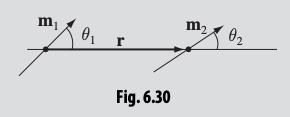
\includegraphics[width=0.5\textwidth]{hw11_1.png}
    \end{figure}
    From the figure above,
    \begin{align*}
        \vb m_1 \vdot \vb m_2 &= m_1 m_2 \cos(\theta_1 - \theta_2) \\
        \vb m_1 \vdot \vu r &= m_1 \cos \theta_1 \\
        \vb m_2 \vdot \vu r &= m_2 \cos \theta_2
    \end{align*}
    And using the cos difference formula
    \[\cos(\theta_1 - \theta_2) = \cos \theta_1 \cos \theta_2 + \sin \theta_1 \sin \theta_2\]
    The interaction energy is
    \begin{align*}
        U &= \frac{\mu_0}{4\pi} \frac{1}{r^3} [m_1 m_2 \cos(\theta_1 - \theta_2) - 3 m_1 m_2 \cos \theta_1 \cos \theta_2] \\
        &= \frac{\mu_0}{4\pi} \frac{1}{r^3} m_1 m_2
            [(\cos\theta_1 \cos\theta_2 + \sin\theta_1 \sin\theta_2) - 3 \cos \theta_1 \cos \theta_2] \\
        &= \frac{\mu_0}{4\pi} \frac{1}{r^3} m_1 m_2
            [\sin\theta_1 \sin\theta_2 - 2 \cos \theta_1 \cos \theta_2] \\
    \end{align*}
    The stable configuration happens when 
    \begin{align*}
        \pdv{U}{\theta_1} = \pdv{U}{\theta_2} = 0
    \end{align*}
    So
    \begin{align*}
        \pdv{U}{\theta_1} &= \frac{\mu_0}{4\pi} \frac{1}{r^3} m_1 m_2
            [\cos\theta_1 \sin\theta_2 + 2 \sin \theta_1 \cos \theta_2] = 0 \\
            &\implies 2\sin\theta_1 \cos\theta_2 = - \cos\theta_1 \sin\theta_2
    \end{align*}
    and
    \begin{align*}
        \pdv{U}{\theta_2} &= \frac{\mu_0}{4\pi} \frac{1}{r^3} m_1 m_2
            [\sin\theta_1 \cos\theta_2 + 2 \cos \theta_1 \sin \theta_2] = 0 \\
            & \implies 2\cos\theta_1 \sin\theta_2 = - \sin\theta_1 \cos\theta_2
    \end{align*}
    Which implies that both
    \begin{align*}
        \sin\theta_1 \cos\theta_2 = \cos\theta_1 \sin\theta_2 = 0
    \end{align*}
    or two sets of solutions
    \begin{align*}
        \sin\theta_1 = \sin\theta_2 = 0 \qor \cos\theta_1 = \cos\theta_2 = 0
    \end{align*}
    For the first set, we can have either $\theta_1 = \theta_2 = 0$ (aligned horizontal dipoles $\rightarrow \rightarrow$) or
    $\theta_1 = 0 \qand \theta_2 = \pi$ (anti aligned horizontal dipoles $\rightarrow \leftarrow$), but for the anti aligned
    case, the magnetic field $\vb B_2$ will not be parallel to $\vb m_1$ so it is not a stable configuration.
    
    For the second set, we can have either $\theta_1 = \theta_2 = \frac{\pi}{2}$ (aligned vertical dipoles $\uparrow \uparrow$) or
    $\theta_1 = \frac{\pi}{2} \qand \theta_2 = -\frac{\pi}{2}$ (anti aligned vertical dipoles $\uparrow \downarrow$), but for the aligned case,
    the magnetic field $\vb B_2$ will not be parallel to $\vb m_1$ so it is not a stable configuration.

    Therefore, looking at the two stable configurations:
    \begin{align*}
        U_{\rightarrow \rightarrow} &= \frac{\mu_0}{4\pi} \frac{1}{r^3} m_1 m_2 [
            \sin 0 \sin 0 - 2 \cos 0 \cos 0
        ] \\
        &= \frac{\mu_0}{4\pi} \frac{1}{r^3} m_1 m_2 [-2] \\
        U_{\uparrow \downarrow} &= \frac{\mu_0}{4\pi} \frac{1}{r^3} m_1 m_2 \qt[
            \sin \frac{\pi}{2} \sin \frac{-\pi}{2} - 2 \cos \frac{\pi}{2} \cos \frac{-\pi}{2}
        ] \\
        &= \frac{\mu_0}{4\pi} \frac{1}{r^3} m_1 m_2 [-1]
    \end{align*}
    So the lower energy is the more stable configuration
    \begin{align*}
        U_{\rightarrow \rightarrow} < U_{\uparrow \downarrow}
    \end{align*}
    thus the dipoles line up horizontally parallel $\rightarrow \rightarrow$.

    \item [(d)] If a bunch of compasses were lined up along a straight line, they 
    would align in straight line similarly to part (c): $\rightarrow \rightarrow \rightarrow \dots$
\end{itemize}

\newpage
\paragraph{7.1}
% hw11_2.png
\begin{figure}[ht]
    \centering
    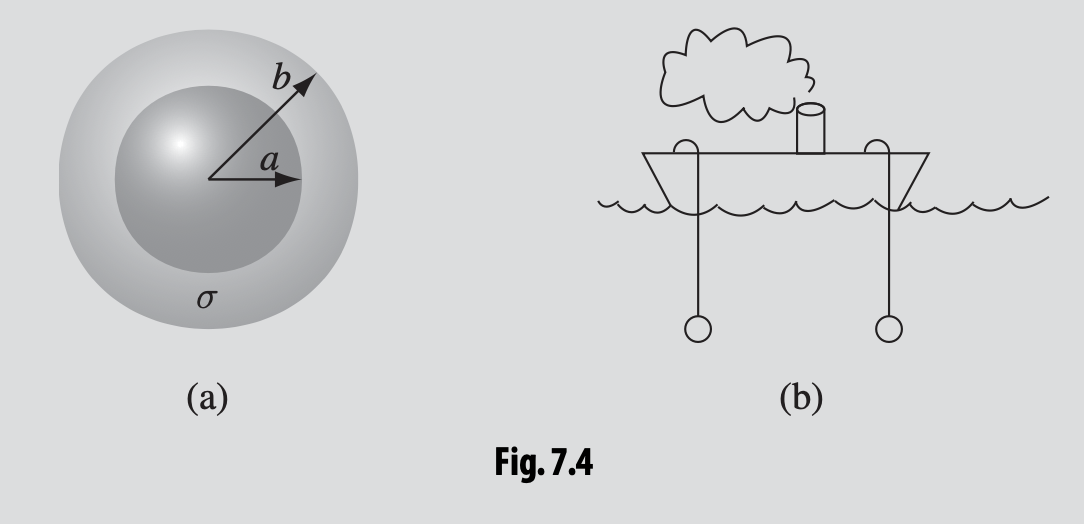
\includegraphics[width=0.5\textwidth]{hw11_2.png}
\end{figure}
\begin{itemize}
    \item [(a)] Between the two shells we have an electric field
    \begin{align*}
        \vb E &= \ke \frac{Q}{r^2} \vu r
    \end{align*}
    So we have a potential difference
    \begin{align*}
        V &= -\int_b^a \vb E \cdot \dd{\vb l} \\
        &= -\ke Q \int_b^a \frac{1}{r^2} \dd{r} \\
        &= -\ke Q \qt(
            -\frac{1}{a} + \frac{1}{b}
        ) \\
        &= \ke Q \qt(
            \frac{1}{a} - \frac{1}{b}
        ) \\
        \implies & Q = \frac{4\pi\epsilon_0 V}{1/a - 1/b}
    \end{align*}
    The current is therefore
    \begin{align*}
        I &= \int \vb J \cdot \dd{\vb a} = \sigma \int \vb E \cdot \dd{\vb a}
        = \frac{\sigma}{\epsilon_0} Q \\
        &= \frac{\sigma}{\epsilon_0} \frac{4\pi\epsilon_0 V}{1/a - 1/b} \\
    \end{align*}
    or
    \begin{align*}
        \boxed{I = \frac{4\pi\sigma V}{1/a - 1/b}}
    \end{align*}
    \item [(b)] The resistance between the shells is
    \begin{align*}
        \boxed{R = \frac{V}{I} = \frac{1}{4\pi\sigma} \qt(
            \frac{1}{a} - \frac{1}{b}
        )}
    \end{align*}
    \item [(c)] If $b \gg a$, $\frac{1}{b} \to 0$ so the resistance is simply
    \begin{align*}
        R = \frac{1}{4\pi\sigma a}
    \end{align*}
    For two shells immersed really deep in the sea with potential difference $V$, the
    we can add the resistance in series i.e.
    \begin{align*}
        R_\text{sea} = 2 \times \frac{1}{4\pi\sigma a} = \frac{1}{2\pi\sigma a}
    \end{align*}
    Thus the current flowing between the two metal spheres is
    \begin{align*}
        \boxed{I = \frac{V}{R_\text{sea}} = 2\pi\sigma a V}
    \end{align*}
\end{itemize}

\newpage
\paragraph{7.2}
% hw11_3.png
\begin{figure}[ht]
    \centering
    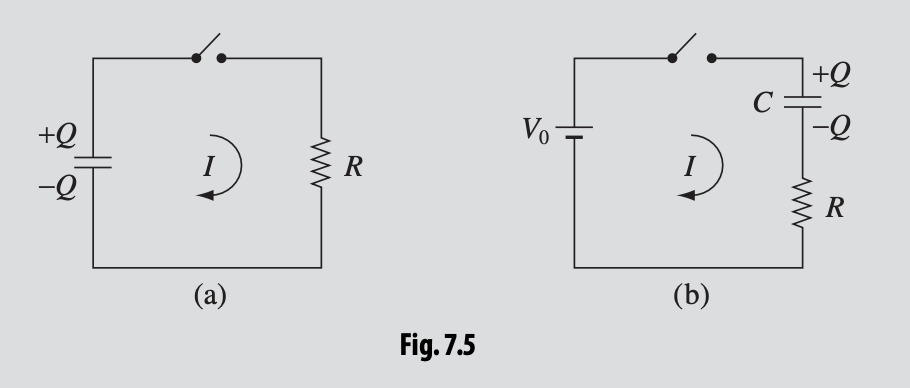
\includegraphics[width=0.5\textwidth]{hw11_3.png}
\end{figure}
\begin{itemize}
    \item [(a)] Inititally, $V_0 = \frac{Q_0}{C}$ As the capacitor discharges the current decreases,
    \begin{align*}
        \dv{Q}{t} &= -I
    \end{align*}
    and the sum of the voltages across the capacitor and the resistor is
    \begin{align*}
        \sum V &= V_C + V_R = 0 \\
        &= \frac{Q}{C} + IR \\
        \implies \dv{Q}{t} &= -I = -\frac{Q}{RC} \\
    \end{align*}
    The solution to this differential equation $\dv{Q}{t} = -kQ$ is
    \begin{align*}
        Q(t) &= Q_0 e^{-kt} \\
        \implies I(t) &= -\dv{Q}{t} = -kQ_0 e^{-kt} \\
        &= -\frac{Q_0}{RC} e^{-t/RC}
    \end{align*}
    and from the initial condition $Q_0 = CV_0$,
    \begin{align*}
        \boxed{
            I(t) = -\frac{V_0}{R} e^{-t/RC}
        }
    \end{align*}
    \item [(b)] The original energy stored in the capacitor is (2.55)
    \begin{align*}
        \boxed{W = \frac{1}{2} CV_0^2}
    \end{align*}
    So integrating the power equation (7.7)
    \begin{align*}
        \int_0^\infty P &= \int_0^\infty I^2 R \dd{t} \\
        &= \frac{V_0^2}{R} \int_0^\infty e^{-2t/RC} \dd{t} \\
        &= \frac{V_0^2}{R} \qt[
            -\frac{RC}{2} e^{-2t/RC}
        ]\eval_0^\infty \\
        &= \frac{V_0^2}{R} \qt[
            0 + \frac{RC}{2}
        ] \\
        &= \frac{1}{2} CV_0^2
    \end{align*}
    \item [(c)] Initially connecting the battery of $V_0$:
    \begin{align*}
        V_0 &= \sum V = V_C + V_R = \frac{Q}{C} + IR
    \end{align*}
    where the current will start to increase, $\dv{Q}{t} = I$, so
    \begin{gather*}
        V_0 = \frac{Q}{C} + R \dv{Q}{t} \\
        CV_0 = Q + RC \dv{Q}{t} \\
        \implies \dv{Q}{t} = \frac{C V_0 - Q}{R C} \\
    \end{gather*}
    And rewriting to get $-1/RC$ on to the right side:
    \begin{align*}
        \dv{Q}{t} = -\frac{Q - C V_0}{RC} \\
        \frac{\dd{Q}}{Q - C V_0} = -\frac{\dd{t}}{RC} \\
    \end{align*}
    Integrating both sides
    \begin{align*}
        \ln(Q - C V_0) &= -\frac{t}{RC} + k \\
        Q - C V_0 &= e^{-t/RC + k} \\
        Q &= C V_0 + e^{-t/RC + k} \\
        \implies Q(t) &= C V_0 + ke^{-t/RC}
    \end{align*}
    And from the initial condition $Q(0) = 0$,
    \begin{align*}
        Q(0) &= C V_0 + k = 0 \\
        \implies k &= -C V_0
    \end{align*}
    So the charge on the capacitor is
    \begin{align*}
        \boxed{Q(t) = C V_0 (1 - e^{-t/RC})}
    \end{align*}
    and the current is
    \begin{align*}
        I(t) &= \dv{Q}{t} = CV_0 \qt(\frac{1}{RC} e^{t/RC}) = \boxed{
            \frac{V_0}{R} e^{-t/RC} 
        }
    \end{align*}
    \item [(d)] Integrating power to get the energ from the battery:
    \begin{align*}
        \int P &= \int_0^\infty IV_0 \dd{t} \\
        &= \frac{V_0^2}{R} \int_0^\infty e^{-t/RC} \dd{t} \\
        &= \frac{V_0^2}{R} \qt[
            -RC e^{-t/RC}
        ]\eval_0^\infty \\
        &= \frac{V_0^2}{R} \qt[
            0 + RC
        ]= \boxed{CV_0^2}
    \end{align*}
    The heat delivered to the resistor is still $\boxed{\frac{1}{2} CV_0^2}$, so the final energy
    stored in the capacitor is $\boxed{\frac{1}{2} CV_0^2}$ i.e. 50\% of the work done by the
    battery shows up as energy in the capacitor.
\end{itemize}

\paragraph{7.7} Magnetic field points into the page
% hw11_4.png
\begin{figure}[ht]
    \centering
    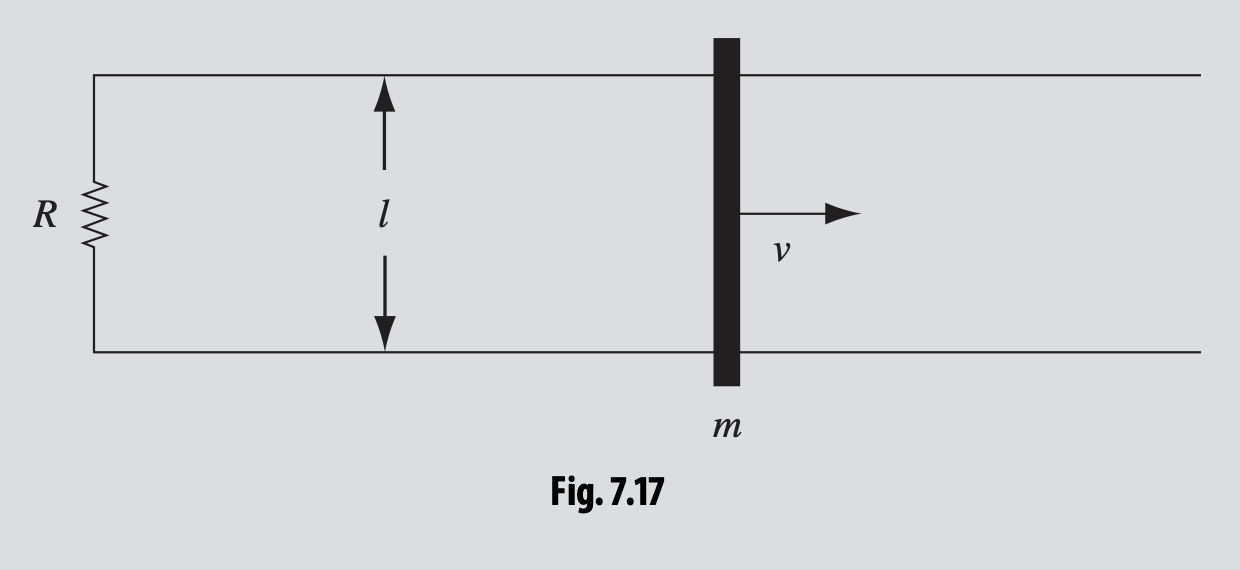
\includegraphics[width=0.5\textwidth]{hw11_4.png}
\end{figure}
\begin{itemize}
    \item [(a)] If the bar moves to the right with speed $v$ the EMF is
    \begin{align*}
        \mathcal{E} &= B \ell v
    \end{align*}
    And since $\mathcal{E} = IR$, the current is
    \begin{align*}
        \boxed{I = \frac{B \ell v}{R}}
    \end{align*}
    where RHR points upwards (or counterclockwise) so the current points downwards in the resistor.
    \item [(b)] The magnetic force on the bar is
    \begin{align*}
        \boxed{F = I\ell B = \frac{B^2 \ell^2 v}{R}}
    \end{align*}
    and from RHR, the force points left
    \item [(c)] Starting at speed $v_0$ at $t=0$, to find the speed at later time $t$ we can
    just use Newton's second law
    \begin{gather*}
        F = m \dv{v}{t} = -\frac{B^2 \ell^2 v}{R} \\
        \dv{v}{t} = \qt(\frac{B^2 \ell^2}{mR}) v \qor \dv{v}{t} = - kv \\
        \implies v(t) = v_0 e^{-kt} = \boxed{v_0 e^{-\frac{B^2 \ell^2}{mR} t}}
    \end{gather*}
    \item [(d)] Given the initial kinetic energy $\frac{1}{2} mv_0^2$, and we can check this by 
    integratin the power to get the work done by the magnetic field
    \begin{align*}
        \int_0^\infty P \dd{t} &= \int_0^\infty I^2 R \dd{t} \\
        &= \frac{B^2 \ell^2}{R} v_0^2 \int_0^\infty e^{-2kt} \dd{t} \quad k = \frac{B^2 \ell^2}{mR} \\
        &= \frac{B^2 \ell^2}{R} v_0^2 \qt[
            -\frac{1}{2k} e^{-2kt}
        ]\eval_0^\infty \\
        &= \frac{B^2 \ell^2}{R} v_0^2 \qt[
            0 + \frac{1}{2k}
        ] \\
        &= \frac{1}{2} m v_0^2
    \end{align*}
\end{itemize}

\newpage
\paragraph{7.8} 
% hw11_5.png
\begin{figure}[ht]
    \centering
    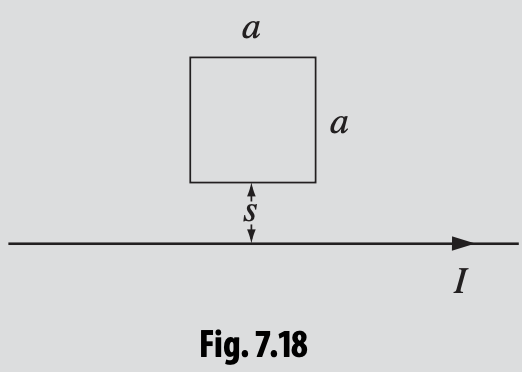
\includegraphics[width=0.3\textwidth]{hw11_5.png}
\end{figure}
\begin{itemize}
    \item [(a)] The flux of $\vb B$ through the loop: From HW 5b, the magnetic field of a long 
    straight wire is 
    \begin{align*}
        \vb B = \frac{\mu_0 I}{2\pi r} \vu \phi
    \end{align*}
    So the flux is simply the integral
    \begin{align*}
        \Phi = \int \vb B \vdot \dd{\vb a}
    \end{align*}
    where the surfance element is $\dd{\vb a} = a \dd{s}$ from $s \to s + a$:
    \begin{align*}
        \Phi &= \frac{\mu_0 Ia }{2\pi} \int_s^{s+a} \frac{1}{s} \dd{s} \\
        &= \boxed{\frac{\mu_0 Ia}{2\pi} \ln\qt(\frac{s+a}{s})}
    \end{align*}
    \item [(b)] If the loop is moved away from the wire at velocity $v$, the EMF is
    \begin{align*}
        \mathcal{E} &= -\dv{\Phi}{t} = -\dv{t} \frac{\mu_0 Ia}{2\pi} [\ln(s + a) - \ln(s)] \quad \dv{s}{t} = v \\
        &= -\frac{\mu_0 Ia}{2\pi} \qt[
            \frac{v}{s + a} - \frac{v}{s}
        ] \\
        &= \frac{\mu_0 Ia v}{2\pi} \qt[
            \frac{1}{s} - \frac{1}{s + a}
        ] \\
        &= \frac{\mu_0 Ia v}{2\pi} \qt[
            \frac{s+a}{s(s+a)} - \frac{s}{s(s+a)}
        ] \\
        &= \boxed{
            \frac{\mu_0 Ia^2 v}{2\pi s(s+a)}
        }
    \end{align*}
    From RHR $(\vb v \times \vb B)$---$\vb v$ points up and $\vb B$ point out of the page---points to the right,
    but the magitude of force is less on the top side of the loop so the current flows
    counterclockwise.
    \item [(c)] No EMF is generated if the loop is moved parallel to the wire!
\end{itemize}

\end{document}
